\documentclass{sig-alternative}
% \documentclass[conference]{IEEEtran}
\usepackage{color}
\usepackage{listings}
\usepackage{graphicx} 
\usepackage{cite}
\usepackage{paralist}
\usepackage[table,xcdraw]{xcolor}
\usepackage{siunitx}
\usepackage{rotating}
\usepackage{eqparbox}
\usepackage{graphics}
\usepackage{colortbl} 
\usepackage{multirow}
\usepackage{times}
\usepackage{balance}
\usepackage{picture}
\usepackage{algorithm}
\usepackage{algorithmicx}
\usepackage{algpseudocode}
\usepackage[export]{adjustbox}
\renewcommand{\footnotesize}{\scriptsize}
\definecolor{lightgray}{gray}{0.8}
\definecolor{darkgray}{gray}{0.6}
\renewcommand{\algorithmicrequire}{\textbf{Input:}}
\renewcommand{\algorithmicensure}{\textbf{Output:}}
\usepackage[table]{xcolor}
\definecolor{Gray}{rgb}{0.88,1,1}
\definecolor{Gray}{gray}{0.85}
\definecolor{Blue}{RGB}{0,29,193}
\newcommand{\G}{\cellcolor{green}}
\newcommand{\Y}{\cellcolor{yellow}}


\definecolor{MyDarkBlue}{rgb}{0,0.08,0.45} 
\lstset{
    language=Python,
    basicstyle=\ttfamily\fontsize{2.7mm}{0.8em}\selectfont,
    breaklines=true,
    prebreak=\raisebox{0ex}[0ex][0ex]{\ensuremath{\hookleftarrow}},
    frame=l,
    showtabs=false,
    showspaces=false,
    showstringspaces=false,
    keywordstyle=\bfseries,
    emph={furthest,gale,better,improved,where,fastmap,split,project,mutate,mutate1}, emphstyle=\bfseries\color{blue},
    stringstyle=\color{green!50!black},
    commentstyle=\color{gray}\itshape,
    numbers=left,
    captionpos=t,
    escapeinside={\%*}{*)}
}


%%% graph
\newcommand{\crule}[3][darkgray]{\textcolor{#1}{\rule{#2}{#3}}}
%\newcommand{\rone}{\crule{1mm}{1.95mm}}
%\newcommand{\rtwo}{\crule{1mm}{1.95mm}\hspace{0.3pt}\crule{1mm}{1.95mm}}
%\newcommand{\rthree}{\crule{1mm}{1.95mm}\hspace{0.3pt}\crule{1mm}{1.95mm}\hspace{0.3pt}\crule{1mm}{1.95mm}}
%\newcommand{\rfour}{\crule{1mm}{1.95mm}\hspace{0.3pt}\crule{1mm}{1.95mm}\hspace{0.3pt}\crule{1mm}{1.95mm}\hspace{0.3pt}\crule{1mm}{1.95mm}} 
%\newcommand{\rfive}{\crule{1mm}{1.95mm}\hspace{0.3pt}\crule{1mm}{1.95mm}\hspace{0.3pt}\crule{1mm}{1.95mm}\hspace{0.3pt}\crule{1mm}{1.95mm}}
\newcommand{\quart}[3]{\begin{picture}(100,6)%1
{\color{black}\put(#3,3){\circle*{4}}\put(#1,3){\line(1,0){#2}}}\end{picture}}
\definecolor{Gray}{gray}{0.95}
\definecolor{LightGray}{gray}{0.975}
% \newcommand{\rone}{}
% \newcommand{\rtwo}{}
% \newcommand{\rthree}{}
% \newcommand{\rfour}{} 
% \newcommand{\rfive}{}
\newcommand{\wei}[1]{\textcolor{red}{Wei: #1}} 
\newcommand{\Menzies}[1]{\textcolor{red}{Dr.Menzies: #1}} 

%% timm tricks
\newcommand{\bi}{\begin{itemize}}%[leftmargin=0.4cm]}
\newcommand{\ei}{\end{itemize}}
\newcommand{\be}{\begin{enumerate}}
\newcommand{\ee}{\end{enumerate}}
\newcommand{\tion}[1]{\S\ref{sect:#1}}
\newcommand{\fig}[1]{Figure~\ref{fig:#1}}
\newcommand{\tab}[1]{Table ~\ref{tab:#1}}
\newcommand{\eq}[1]{Equation~\ref{eq:#1}}

%% space saving measures

%\usepackage[shortlabels]{enumitem}  
\usepackage{url}
% \def\baselinestretch{1}


% \setlist{nosep}
%  \usepackage[font={small}]{caption, subfig}
% \setlength{\abovecaptionskip}{1ex}
%  \setlength{\belowcaptionskip}{1ex}

%  \setlength{\floatsep}{1ex}
%  \setlength{\textfloatsep}{1ex}
%  \newcommand{\subparagraph}{}

% \usepackage[compact,small]{titlesec}
% \DeclareMathSizes{7}{7}{7}{7} 
% \setlength{\columnsep}{7mm}

\begin{document}
% \conferenceinfo{FSE}{'15 Bergamo, Italy}
\title{ A Little Sampling Goes A Long Way}
\numberofauthors{2}
\author{
        \alignauthor Vivek Nair, Tim Menzies, Xipeng Shen 
        \affaddr{Computer Science, North Carolina State University, Raleigh, USA}
        \email{vivekaxl, tim.menzies, xipengshen@gmail.com}
    \and  
        \alignauthor Norbert Siegmund, Sven Apel \\
        \affaddr{Computer Science, University of Passau, Germany}\\
        \email{norbert.siegmund, apel@uni-passau.de}
       }

\maketitle 
\thispagestyle{plain}
\pagestyle{plain}
\begin{abstract}
Active Learning, Configuration, Sampling, Machine Learning, Performance Prediction


\end{abstract}

% A category with the (minimum) three required fields
\vspace{1mm}
\noindent
{\bf Categories/Subject Descriptors:} 
D.2 [Software Engineering] ;
I.2.6 [Artificial Intelligence]: Induction

 
\vspace{1mm}
\noindent

{\bf Keywords:} Performance prediction, Active Learning, 
Multi-Objective Optimization,
Search-based Software Engineering,Sampling, Machine Learning.

\pagenumbering{arabic} %XXX delete before submission
 
 
\section{Introduction}
 The complexity involving configuring software systems have grown over the recent years \cite{berger2013study}. A configurable system provides configuration options to customize a software system to a given set of requirements. 
 A configuration option is related to a certain feature of the software system and state of the configuration system defines whether the feature is  active in the system.
 For e.g. The state of the configuration option ITracing of  Berkeley DB Java controls whether tracing is turned on/off (citation). Not all combinations of features can be used(generally) and there are constraints, which needs to be followed while configuring a system. These constraints are defined by a \textit{Feature Model}\cite{kang1990feature} or \textit{Decision Model}\cite{schmid2011comparison}. 
 
 In order for the users to decide on an optimal configuration for a particular job/functionality, they need an understanding of the dependencies between various configuration or perform an exhaustive search of all the configuration options. Exhaustive search is very time consuming given that n number of configuration will result in $2^n$ number of configurations. To reduce the time required to find an optimal configuration, the key challenge is to build a model of the software system using only a small number of sample configuration, in such a way that it can accurately predict the performance of the software system. This model can be then used to find the optimal configuration using a meta-heuristic algorithm like GALE etc. 
 

 
Our goal is to build performance models that can be build using the few training samples, which then can be used to find optimal configuration of the system (minimize run time of a job). Our work was motivated by the fact that in real world scenario, cost of acquiring optimal configuration is expensive and time consuming \cite{weiss2008maximizing}. To further emphasize that it is expensive to collect complete configuration space (exhaustive search), let us look at an example. Assume that there is a software system with 9 features (configuration space = $2^9$) and a job requires at an average 20 minutes to execute. The total time required to find an optimal configuration, using exhaustive search, is 4300 minutes ($2^9 \times 20$). This problem can be solved in a short amount of time, if the user can build a performance model with fewer samples ($\ll 2^n$). From a learner perspective, our goal can be described as a sampling technique, which can determine "good sample" for a given system. A "good sample" can be described as a sample if it is small enough to decrease the measurement effort and large enough to increase the prediction accuracy of the model. We propose two new sampling techniques, which uses a clustering technique and use point/s from clusters to build the sample. We conduct experiments on six real-world configurable system to compare the sampling strategies in terms of total time saved by the sampling techniques wrt. to the baseline strategy ($2/3$ of the sample size).

The backbone of the approaches presented in the paper can be summarized as clustering the configurable space and select members from the cluster in such as way that those points are representative of the whole cluster. We tried to validate the sampling techniques by answering the following questions:
        \bi
            \item{RQ1: Can a reasonable prediction accuracy be achieved based on subset of a training set?}
            \item{RQ2: Does less data used in building the models lead to large variance in the predicted values?}
            \item{RQ3: Can evolutionary algorithms be used to find the optimal configurations using the model generated?}
        \ei
 
\section{Bird's Eye Overview}


    \textbf{Sampling: } Figure ~\ref{fig:GeneralProcess} illustrates the general process of performance prediction using sampling. It starts with an initial sample of measured configurations, which are used to build the prediction model. A good initial sample significantly reduces the effort involved with training sample collection. The state of the art approaches involves progressive and projective sampling techniques \cite{sarkar2015cost} and Fourier Transforms \cite{zhang2015performance}. However these approaches assumes the user to know a lot of about the system, which is not a fair assumption. The problem with iterative techniques lies in the step size, which is an engineering decision(aka black art). In our approach, we use clustering, which uses the first principle component, to determine clusters rather than relying to random sampling methods. Once the clusters are obtained, \'interesting\' representative/s from each cluster  is/are collected. Then these points are used to build prediction models using a statistical learning technique called Classification and Regression Tree (CART), which has been demonstrated to be fast and accurate for performance prediction of configurable system \cite{guo2013variability}.
    
In our work, we use the time saved by the proposed sampling when compared to the exhaustive search is presented along with the prediction accuracy (similar to ~\cite{guo2013variability}, \cite{siegmund2012predicting}, \cite{westermann2012automated}). 
    \begin{figure}[!t]
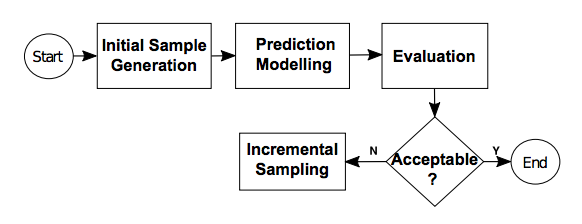
\includegraphics[width=0.9\linewidth]{Figures/GeneralProcess.png}
\caption{ General Process of Performance Modelling }\label{fig:GeneralProcess}
\end{figure}


    \textbf{Search Algorithms: }Linear time algorithms works well, when the problem scenario is same as the scenarios where the algorithm was developed. But in the real work scenario, the scenarios presented are slightly different from what the algorithms were developed in. For example, one particular technique is available to calculate the minimum-cost allocation of resources for a problem where both the cost function and constraints are linear. The method is fast and reliable. And it is almost applied inappropriately  in real-world settings where the cost function and constraints are almost always nonlinear. In essence, anyone using this method runs the risk of generating the right answer to a problem that does not exist \cite{michalewicz2013solve}. 
    Another challenge faced by the deterministic algorithms lie in the fact the each new solution
relies on a single solution as the basis for future exploration with each iteration. They either process complete solutions in their entirety, or they construct the final solution from smaller building blocks. Greedy algorithms,
Dynamic programming, Branch and bound methods etc. 

Evolutionary algorithms abandons this idea totally and considers multiple solutions at the same time. Evolutionary algorithm starts with an \textit{initial population} (randomly generated, based on some constraints). Since the solutions are drawn from a uniform distribution, typically, this diversity is desirable, although in some cases we might want to initialize all of the available parents to some best-known solution and proceed from there. The chosen \textit{evaluation function} must be capable of differentiating
between two individuals, i.e., it has to be able to rank one solution ahead
of another. Those solutions that are better, as determined by the evaluation
function, are favored to become parents for the next generation of offspring. 
\textit{Reproduction} refers to  new solutions being generated probabilistically in the neighborhood of old solutions. This process continues till the a \"good enough\" solution is achieved or a hard limit on iterations are reached. This criteria is called the \textit{stopping criteria}.
    
    There has been extensive research in evolutionary algorithms in the recent decades. For example, here is a list of search algorithms used widely in research: \textit{simulated annealing}\cite{bell2013limited, menzies2007business}; various genetic algorithms\cite{goldberg1979complexity} agumented by techniques such as \textit{differential evolution} \cite{storn1997differential}, \textit{tabu search and scatter search}\cite{nebro2008abyss, molina2007sspmo, glover1986general, beausoleil2006moss}; \textit{particle swarm optimization}\cite{pan2008particle}; numerous decomposition approaches that use heuristics to decompose the total space into small problems, then apply a response surface methods\cite{krall2014gale, zuluaga2013active}. GALE, short for Geometric Active Learning Evolution,
combines spectral learning and response surface methods
to reduce the number of evaluations needed to assess a set
of candidate solutions. The algorithm is an active learner;
i.e. instead of evaluating all instances, it isolates and explores
only the most informative ones. We explain the working of GALE in section 5.




\section{Problem Formulation}


    Configurations of a software system may not be independent, such that we cannot measure arbitrary configurations. Researchers have explored the presence of complex domain dependencies. With constraint between features, in theory there can be multiple minimal configuration (for example, in the presence of mutually exclusive features). These dependencies are captured well by \textit{Feature Models(FM)}. FM defines all the N features and all the valid configurations C of a software system. Figure ~\ref{fig:bdbc}  shows the feature model of Berkeley DB(C Version) using the notations defined in ~\cite{kang1990feature}, ~\cite{guo2012consistency}. Feature models are used to check the validity of new mutated solutions generated by the learners (eg. GALE).
    
\begin{figure}[!t]
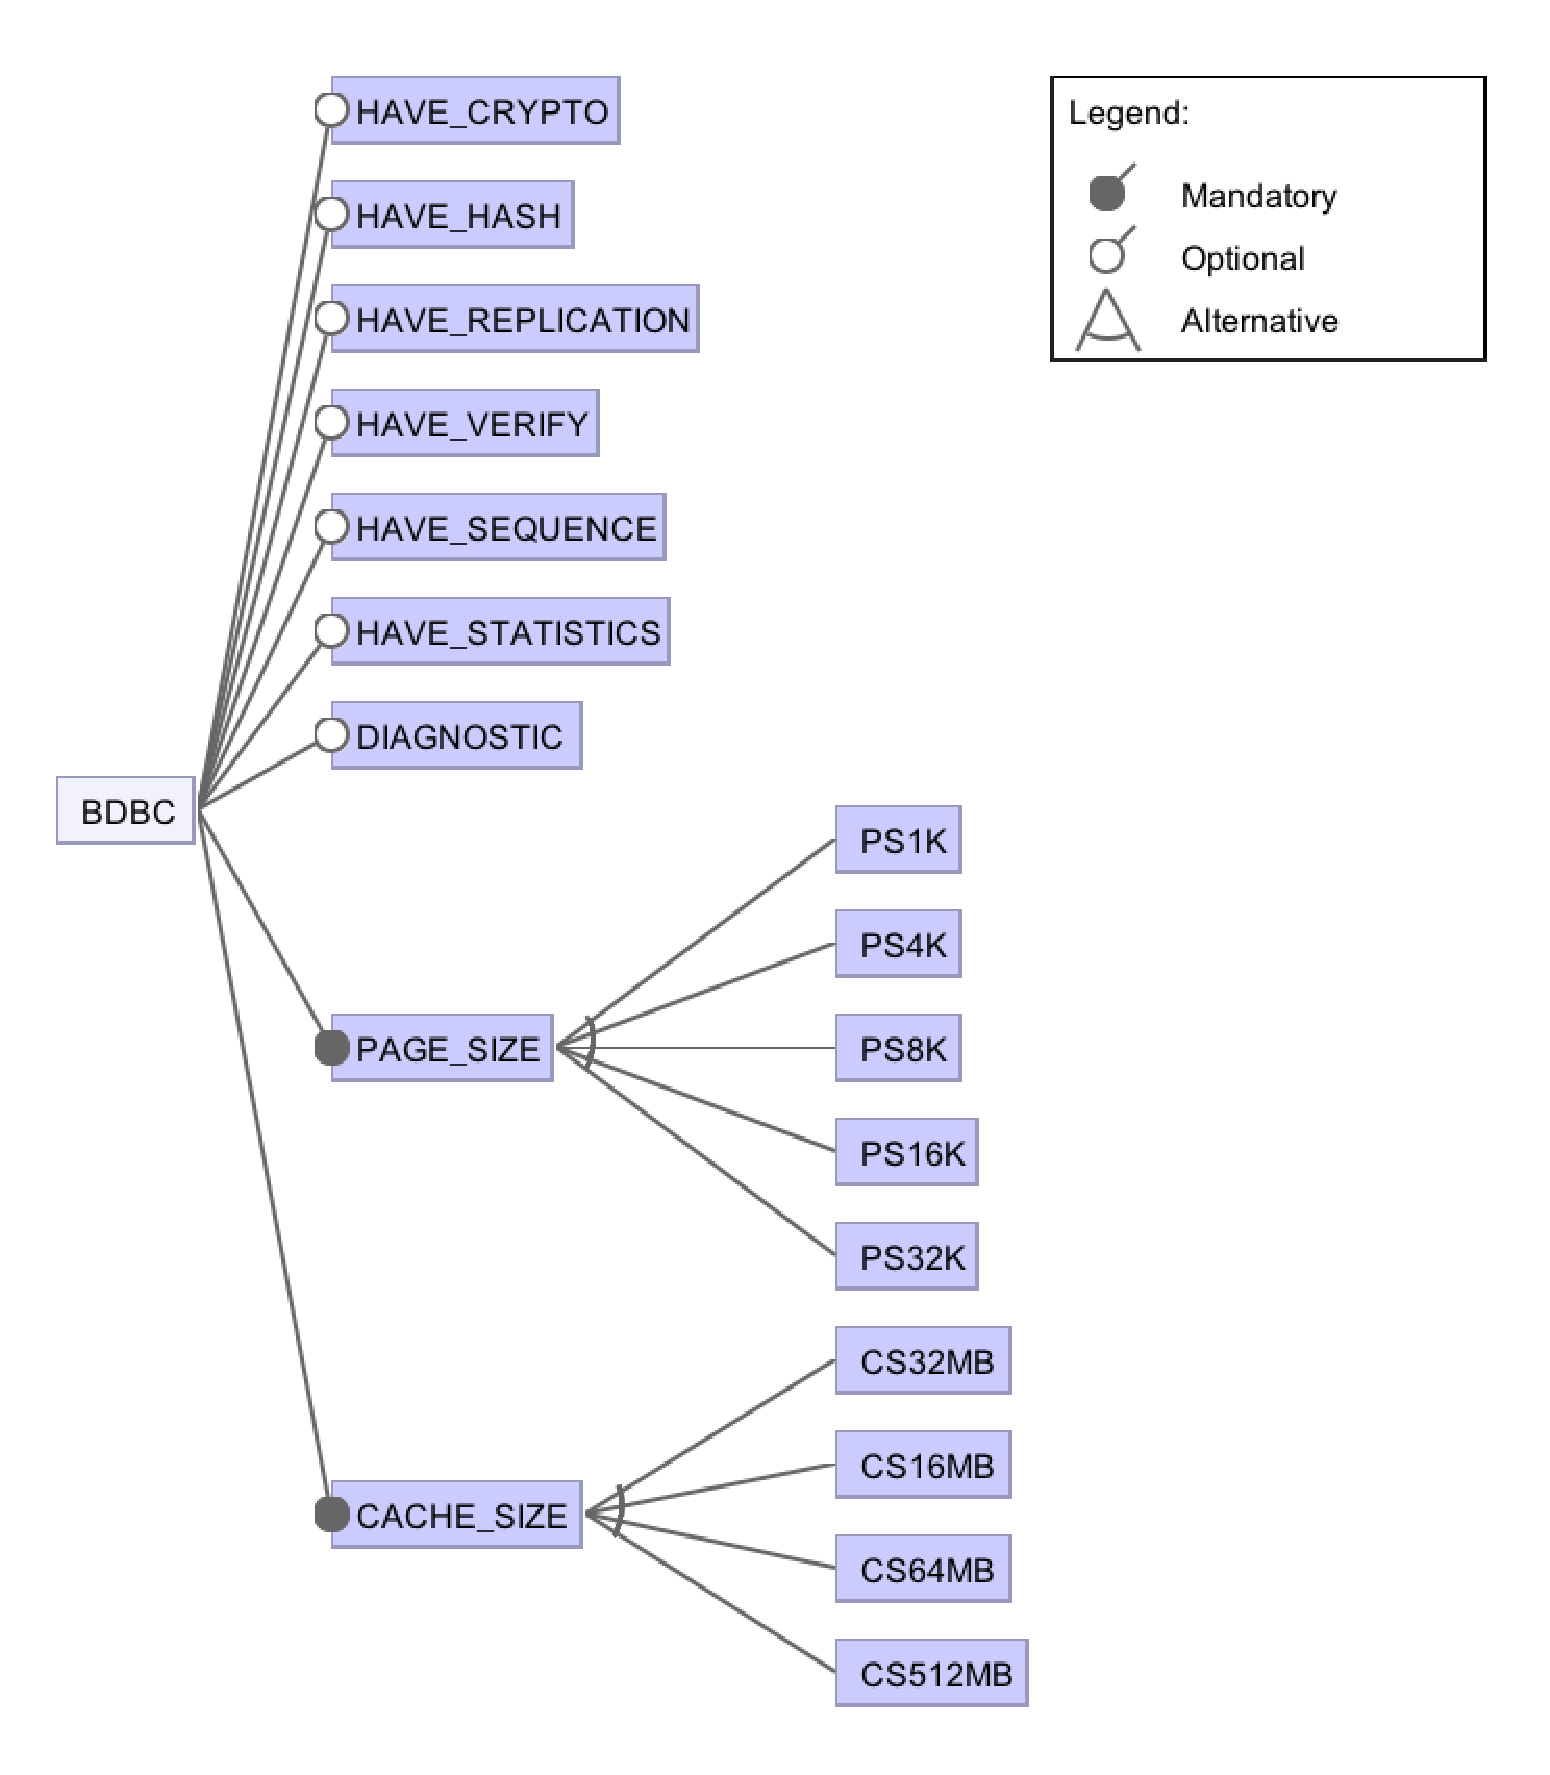
\includegraphics[width=0.9\linewidth]{Figures/BDBC.eps}
\caption{ Berkeley database feature model   (``C'' version). }\label{fig:bdbc}
\end{figure}
    
    The features on the software system is represented as a set of binary decision variables. A feature, when turned on, corresponds to 1, and 0 otherwise. All the features of a system is represented a vector F = $<f_1, f_2, ...,f_N>$, where N is the number of features of the software system. The dependent variable corresponding to a configuration(F) is a performance score, P(F), which the performance measurement.

    Performance of system can be modelled using the configuration as the independent variable and the performance metric as a dependent variable. 
    Modelling a software system is to find a hypothesis function(h), such that h(F) predicts P(F) accurately. This can be represented as:\\
\begin{center}
    $ h: C \mapsto \rm I\!R$ s.t. $L(h(F), P(F))$ is minimized\\
\end{center}

where, L is a loss function for penalizing errors in prediction. By formulating the performance prediction using the method described, we can transform the problem into a learning problem. 
    It should be noted that though the number of possible configurations (C) is equal to $2^N$(binary decision variables), in reality valid configurations(\^{C}) is smaller than C (|C| << |\^C|). 


To answer our research questions, we use data set from our previous work on detecting performance interactions~\cite{SKR+12}. It contains performance measurements of real-world configurable software systems.
These systems were selected to cover a broad range of domains (databases, Web servers, video encoder, compiler), programming languages (C, C++, Java), and different sizes regarding number of features and configurations. Table~\ref{tab:subjectsystems} provides an overview of these systems.
 
 \begin{table}[!t]
\scriptsize
\begin{tabular}{llllll}
  \hline
Project & Domain & Lang. & LOC & Features & Config\\\hline
BDBC: Berkeley DB   & Database & C & 219,811 & 18 & 2560\\
BDBJ: Berkeley DB   & Database & Java & 42,596 & 32  & 400\\
Apache & Web Server & C & 230,277 & 9 & 192\\
SQLite & Database & C & 312,625 & 39 & 3,932,160\\
LLVM & Compiler & C++ & 47,549 & 11 & 1024\\
x264 & Video Enc. & C& 45,743 & 16 & 1152\\\hline
\end{tabular}
 \label{tab:subjectsystems}
\caption{Siegmund data.
For SQLite, the data  contains 4,553 configurations for prediction modeling and 100 additional random configurations for prediction evaluation, see \cite{vapp}.}\label{fig:cpm}
\end{table}

In detail, we use the following systems in our experiments:
\begin{compactitem}
\item \textbf{Berkeley DB CE} is an embedded database system written in C. It is one of the most deployed databases in the world due to its low binary footprint and its configuration abilities. We used the benchmark provided by the vendor to measure response time.
\item \textbf{Berkeley DB JE} is a complete re-development in Java with full SQL support. Similarly, we used a benchmark provided by the vendor measuring response time.
\item \textbf{Apache} is a prominent open-source Web server that comes with various configuration options. To measure performance, we used the tools autobench and httperf to generate load on the Web server. We increased the load until the server could not handle any further requests and marked the maximum load as the performance value.
\item \textbf{SQLite} is an embedded database system deployed over several millions of devices. It supports a vast number of configuration options in terms of compiler flags. As benchmark, we used the benchmark provided by the vendor and measured the response time.
\item \textbf{LLVM} is a compiler infrastructure written in C++. It provides configuration options to tailor the compilation process. As benchmark, we measured the time to compile LLVM's test suite.
\item \textbf{x264} is a video encoder in C that provides configuration options to adjust output quality of encoded video files. As a benchmark, we encoded the Sintel trailer (735\,\%MB) from avi to the xH.264 codec and measured encoding time.
\end{compactitem}
The data in these
data sets have a continuous class (run time of the compiled system)
so the performance of a quality predictor can be measured in terms
of difference between the predicted runtime $p$ of test case items
and their actual runtimes $a$ using 

\begin{equation}\label{eq:1}
MRE = \frac{abs(s-a)}{a} \times 100
\end{equation}


For all systems, except for SQLite, we obtained the whole population data (i.e., all valid configurations). For SQLite, we measured all configurations corresponding to one-way and two-way interactions and additionally sampled 100 random configurations.

\section{Sampling Technique: East-West Where}
\begin{figure}[!t]
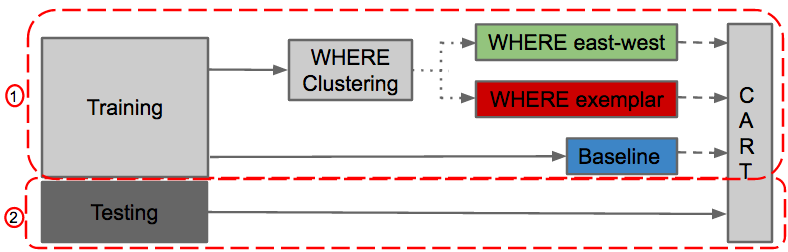
\includegraphics[width=0.9\linewidth]{Figures/SamplingProcess.png}
\caption{Description of Sampling Process. Part 1 describes the training process where as, part 2 describes the testing process.}\label{fig:Sampling Process}
\end{figure}
\subsection{Approach}
This section describes how a large space of candidate solutions (configurations) is clustered into many smaller clusters.
\subsubsection{WHERE Learning}\label{sec:spectral}


WHERE is a {\em spectral learner}~\cite{kamvar2003spectral}; i.e. given solutions with $d$ possible decisions(features), it re-expresses those $d$ decision variables in terms of the $e$ eigenvectors of that data.
This speeds up the reasoning since we then only need to explore the $e\ll d$   eigenvectors.

A widely-used spectral learner is a principal components analysis (PCA). For example, PDDP ({\em Principal Direction Divisive Partitioning})~\cite{boley1998principal} recursively partitions data according to the median point of data projected onto the first PCA component of the current partition.

WHERE~\cite{me12d} is a linear time variant of PDDP  
that uses FastMap~\cite{Faloutsos1995} to quickly find the first component.
Platt~\cite{platt05} shows that FastMap is a  Nystr\"om algorithm that finds approximations to eigenvectors.
As shown in \fig{fastmapCode} on lines 3,4,5, FastMap  projects all data onto a line connecting two distant points(poles)\footnote{
To define distance, WHERE uses the standard Euclidean distance method proposed by Aha et al.~\cite{aha91}; that is: $dist(x,y)= \sqrt{\sum_{i\in d} (x_i - y_i)^2}/\sqrt{ \left\vert{d}\right\vert }$ where distance is computed on the independent decisions $d$ of each candidate solution; all $d_i$ values are normalized min..max, 0..1; and the calculated distance normalized by dividing by the maximum distance across the $d$ decisions.}. 
FastMap finds these two distant points in near-linear time. 
The search for the poles needs only $O(N)$ distance comparisons (lines 19 to 24).
The slowest part of this search is the sort used to find the median $x$ value (line 10) but even that can be reduced to  asymptotically optimal linear-time via the standard median-selection algorithm~\cite{hoare61}.

\begin{figure}[!t] 
\begin{minipage}{3.2in}
\begin{lstlisting}[mathescape,frame=l,numbers=left]
def fastmap(data): 
  "Project data on a line to 2 distant points"
  z          = random.choose(data)
  east       = furthest(z, data)
  west       = furthest(east, data)
  data.poles = (west,east)
  c          = dist(west,east)     
  for one in data.members: 
    one.pos = project(west,east,c,one)
  data = sorted(data) # sorted by 'pos'
  return split(data)

def project(west, east, c, x): 
  "Project x onto line east to west"
  a = dist(x,west)
  b = dist(x,east)
  return (a*a + c*c - b*b)/(2*c) # cosine rule

def furthest(x,data): # what is furthest from x?
  out, max = x,0
  for y in data:
    d = dist(x,y)
    if d > max: out, max = y, d
  return out

def split(data): # Split at median
   mid = len(data)/2; 
  return data[mid:], data[:mid]
\end{lstlisting}
\caption{Splitting data with FastMap}
\label{fig:fastmapCode}  
\end{minipage}
\end{figure}

FastMap returns the data split into two equal halves.
WHERE recurses on the two halves, terminating when some split has less than $\sqrt{N}$ items. To summarize, the WHERE module of the technique takes data points as inputs and returns log(N) number of clusters.

Next two subsections describes various technique of selecting points in such a way that the point select is an representative of the cluster

\subsubsection{WHERE Exemplar}\label{where_exemplar}
This technique borrows from WHERE spectral learner discussed above and uses the clusters to perform clustering. WHERE splits the data into smaller clusters, each of which is characterized by two distant points (poles). 
 The technique assumes the best point (exemplar) as the representative of each cluster. This technique uses one solution from each cluster(best) and hence $log_2(M)$ number of training examples, where M is the size of the configuration space.

\subsubsection{WHERE East West}\label{where_east_west}
This technique as the above technique is also uses the WHERE spectral learner as a precursor to sampling. 
It is assumed  that the technique only needs to evaluate
the most informative subset consisting of the poles used to
recursively divide the data. The recursive binary division of the solutions(M), and that this technique uses two solutions in each cluster, which means the technique uses only $2log_2(M)$.

\subsubsection{WHERE Random}\label{where_random}
This technique uses WHERE spectral learner to cluster the data points and randomly chooses a point from the clusters. It is assumed that a random point in the cluster can be used as a representative to all the points in cluster. This technique only requires to one evaluation per cluster.




We use the points sampled, using the technique described above, to build the predictive model using the popular machine learning technique called Classification and Regression Tree(CART), which has been extensively used in the literature and has been observed to be fast and accurate~\cite{guo2013variability}.

\subsection{Results}
Our sampling methods are stochastic in nature and hence we have repeated the experiments 20 times to report the variance(which represents stability of our results). 
By conducting experiments on six real-world configurable systems, we aim at answering the following research questions

\textit{A. Can a reasonable prediction accuracy be achieved based on 
subset of a training set?}\\
\\
Figure ~\ref{fig:sampling_accuracy} shows how the variation of the  prediction accuracy wrt. to the size of the training set (used before sampling). The x-axis of the graph represents the percentage of the training set used to train the learner (CART) and the y-axis represents the MRE as defined in equation \ref{eq:1}. The WHERE based sampling techniques are compared to \textit{baseline}.  In our experiments, a low MRE is an indicator of good sampling technique. Our assumption based on the machine learning literature(ref needed) is, as the size of the training set increases the accuracy of the predictor must improve. Using this experiment, we are trying to make a case for 'informative' data samples(as obtained by WHERE east But the point that we are trying to make with this experiment is to show that the quantity of the data doesn't matter but how much information is provided by the examples. In sub-graph 1 (Apache), the WHERE east-west performs as well as the baseline technique, where as WHERE exemplar perform worse than the other techniques for most of the training set sizes. WHERE-exemplar only works well when the 90\% of the data set is available for clustering. Sub-graph 3 shows an very interesting property as the number of training samples available for training increases the accuracy of the predictor decreases (which is counter-intuitive). The results of the WHERE exemplar provides evidence to believe that the solution with the best performance score is not a good representative of the cluster. On the other hand, the poles of a cluster is a indeed a good representative of the cluster.\\~\\




\begin{figure}[!t]
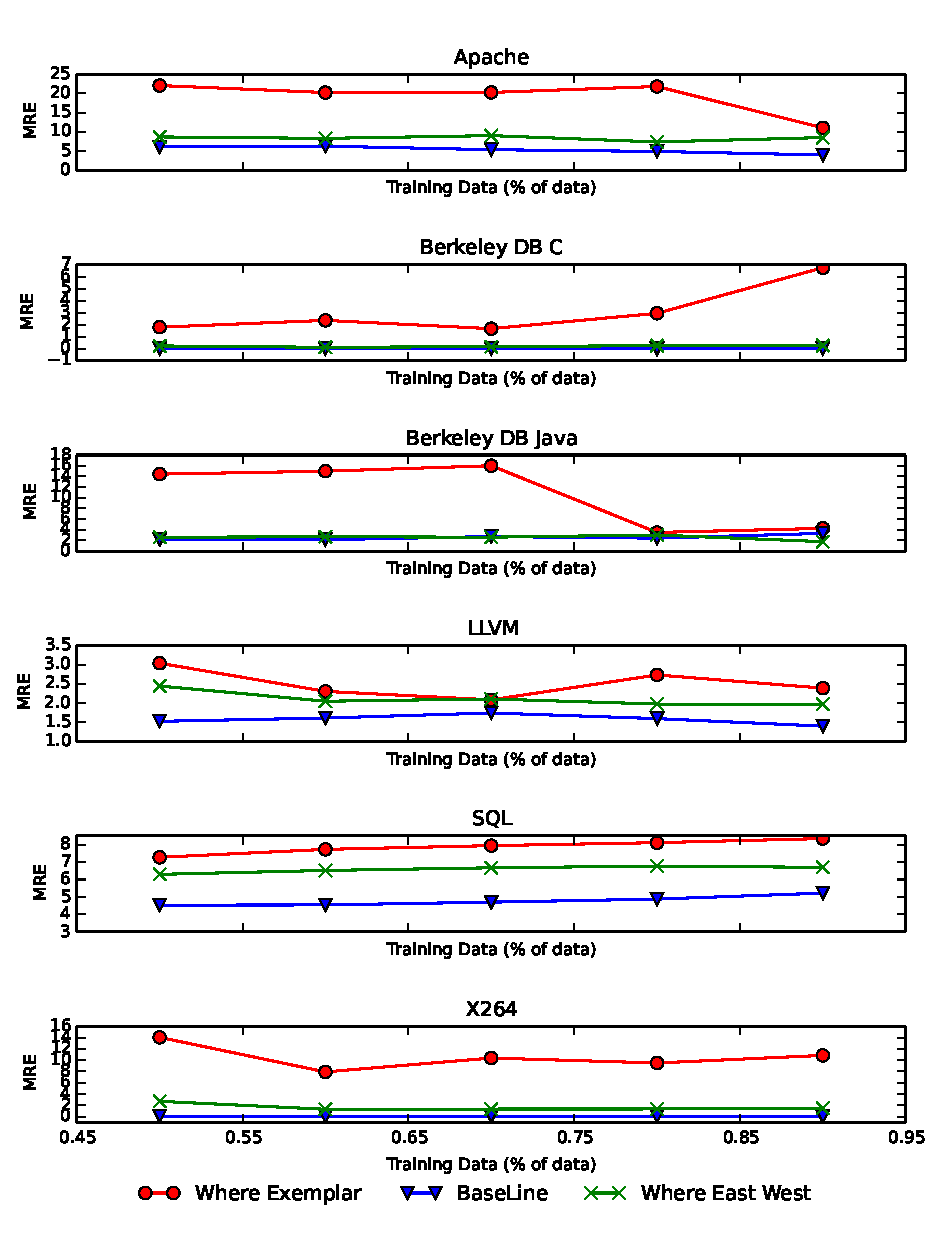
\includegraphics[width=0.9\linewidth]{Figures/SamplingAccuracy.eps}
\caption{Behavior of accuracy of WHERE-exemplar, baseline, WHERE-east-west wrt. to different training set sizes }\label{fig:sampling_accuracy}
\end{figure}

\begin{figure}[!t]
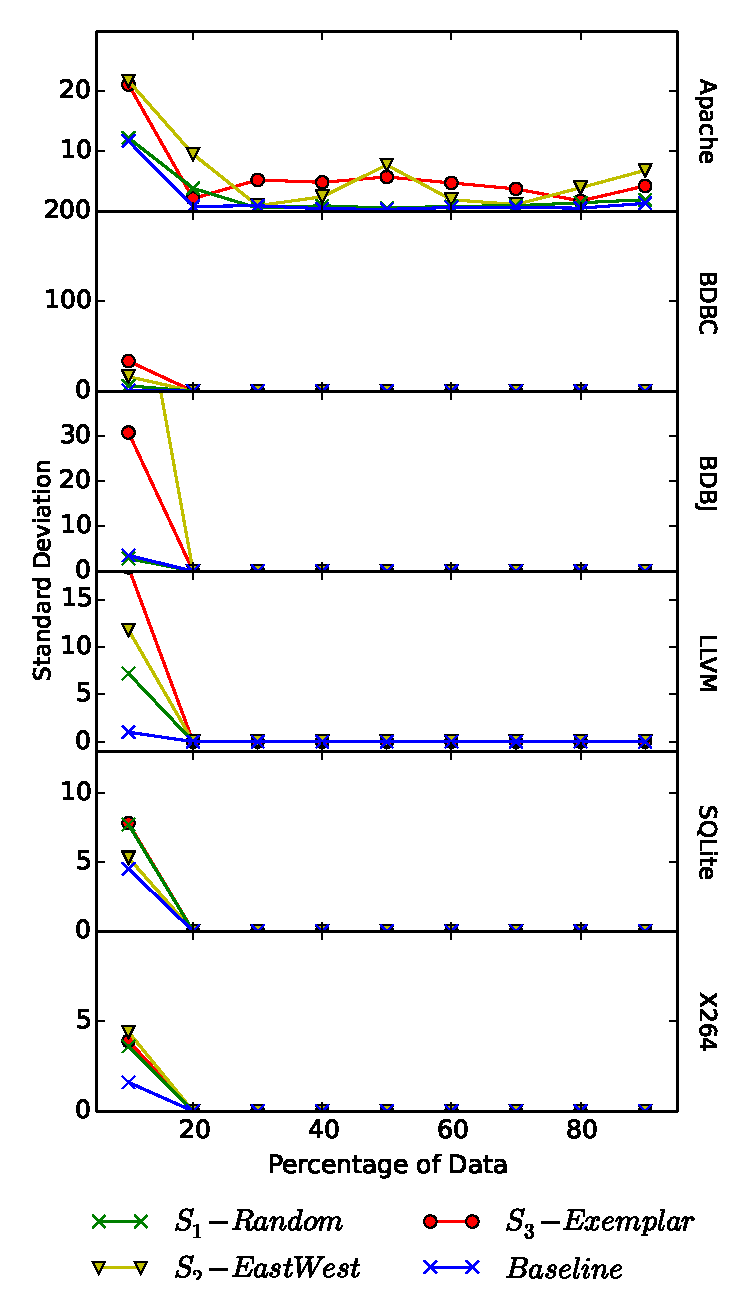
\includegraphics[width=0.9\linewidth]{Figures/Variance.eps}
\caption{Variances }\label{fig:Variance}
\end{figure}

    \begin{figure}[!t]
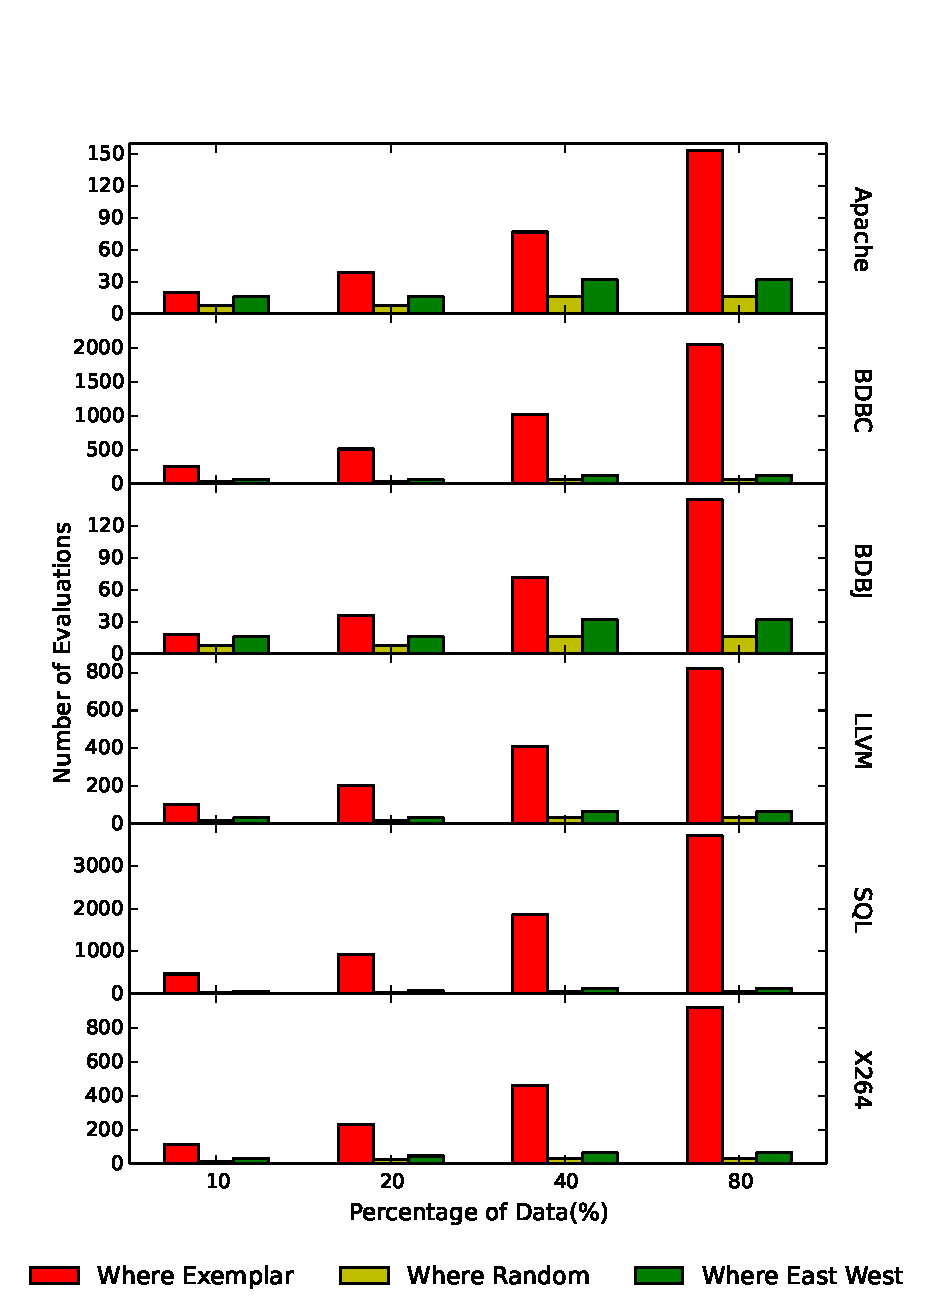
\includegraphics[width=0.9\linewidth]{Figures/evaluation_graph.eps}
\caption{ Comparing evaluations of different approaches }\label{fig:Evaluations}
\end{figure}

    \begin{figure}[!t]
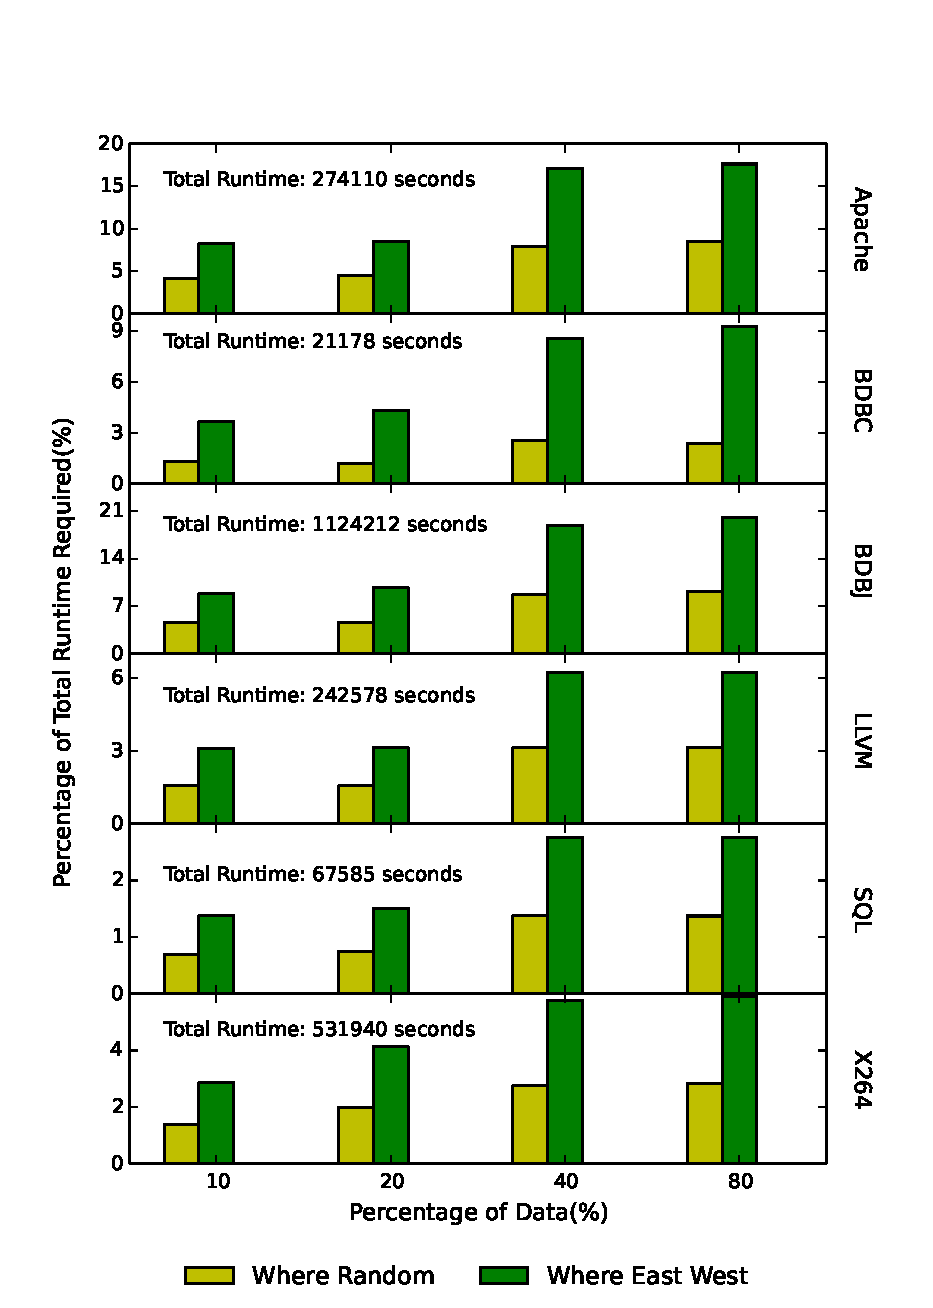
\includegraphics[width=0.9\linewidth]{Figures/sum_of_run_times_graph.eps}
\caption{ Comparing the runtimes of two promising approaches }\label{fig:Runtimes}
\end{figure}


\textit{B. Does less data used in building the models lead to large
variance in the predicted values?}\\

We have shown with sufficient evidence that models can be trained using less data, while achieving the accuracy
attained by using larger training data. 
The another aspect, which needs to be considered at this point is the variability that is introduced  when a sampled dataset used to train CART. 
Figure ~\ref{variance_table} shows the raw scores from the experiment. Each row represents how different techniques(column 1) perform in a dataset(last column). Decimal point numbers on the top of the table represent the percentage of data used to build the CART. The cells highlighted with grey are the cases where the variance is greater than 3\%. The data presented in the table is an evidence to the fact  that \textit{WHERE east-west} doesn't introduce a large variance($[0.23, 2.93]$) where as \textit{WHERE exemplar} is not useful as a sampling technique (this also validates the conclusions drawn in the previous section). 


In Figure \ref{fig:time_saved}, we show the amount of time saved by various sampling methods. The x-axis of the graph represent the percentage of data used to build the CART model. The y-axis shows the time saved by the various sampling methods. There are take away from the figure are:
\bi
    \item{The sampled population remains constant even if the amount of training set increases. This shows that the method is scalable and only depends on the number of features in the dataset rather than the number of rows.}
    \item{From the previous sections, we know that \textit{WHERE east west} achieves 'almost' same accuracy,
    which mean the technique saves time while preserving accuracy and reducing variability.}
\ei


These results, along with the fact that the size of the sampled population is smaller compared to the configuration space, shows us that the \textit{WHERE east west} can indeed save time and effort, when the cost of collecting training samples is expensive.

\section{Fast Searcher: GALE}
Once we have the software performance model build using any sampling technique, the obvious next step is to find the optimal configuration such that the performance score of that particular configuration is the minimal. At this point, we can use any searcher to find the optimal configuration of a system(modelled by CART). In this section, we introduce GALE, which has proven to find near optimal solution with minimum model evaluations as possible. 
\subsection{Approach}
\begin{figure}[!b]
\small
\begin{tabular}{|p{.95\linewidth}|}\hline
GALE initially builds a population of points by selecting decisions at random. It then {\em clusters} those decisions into neighborhoods as follows:
\begin{enumerate}
\item Find two distant points in that population; call them the {\em east} and {\em west} poles. 
\item Draw an axis of length $c$ between the poles. 
\item Let each point be at distance $a,b$ to the {\em east,west} poles.  Using the cosine rule, project each point onto the  axis  at $x=(a^2 + c^2 - b^2)/(2c)$.  
\item Using the median $x$ value, divide the population.
\item For each half that is larger than $\sqrt{N}$ of the original population, go to step 1.
\end{enumerate}

Note that the above requires a distance measure between sets of decisions: GALE uses the standard case-based reasoning measure defined by Aha et al.~\cite{aha91}. Note also that GALE implements step1 via  the FASTMAP~\cite{Faloutsos1995} linear-time
heuristic:
\begin{itemize}
\item Pick any point at random; 
\item Let {\em east} be the point furthest from that point; 
\item Let {\em west} be the point furthest from {\em east}.
\end{itemize}

These final sub-divisions found by this process are the {\em neighborhoods} that GALE will {\em perturb} as follows:
\begin{itemize}
\item Find the objective scores of the {\em east,west} poles in each neighborhood.
\item Using the continuous domination predicate of \fig{moea}, find  the {\em better} pole. 
\item Perturb all points in that neighborhood by pushing them towards the better pole, by a distance  $c/2$ (recall that  $c$ is the distance between the poles).
\item Let generation $i+1$ be the combination of all pushed points from all neighborhoods.
\end{itemize}

From a formal perspective, GALE is an active learner~\cite{Dasgupta2005} that builds a piecewise linear approximation to the Pareto frontier~\cite{Zuluaga:13}.  
For each piece, it then pushes the neighborhood up the local gradient.  This  approximation is built in the reduced dimensional space found the FASTMAP  Nystr\"om approximation to the first component of PCA~\cite{platt05}.
\\\hline
\end{tabular}
\caption{Inside GALE}\label{fig:gale}
\end{figure}
GALE combines (a) the neighborhood perturbation  with (b)~the MOEA algorithm of \fig{moea}.  The algorithm reflects over a {\em population} of points, each of which contains {\em decisions} (configurations of a software system).  It then searches for the input decisions that lead to best outcomes.  For example:
\begin{itemize}
\item we adjust the inputs to CART (modelling the performance score of the software system)
\item GALE can report the best configuration for the system such that the performance score is (near) lowest.
\end{itemize}

\fig{gale} lists the procedure by which GALE clusters the data into neighborhoods, then perturbs each neighborhood.  In terms of monitoring for brittleness, the key point of GALE is that this process continues until the perturbations stop having any new effect (i.e. they stop generating lower performance scores). That is, all GALE solutions are guaranteed not to be brittle.

\begin{figure}[!t]
\small
\begin{tabular}{|p{.95\linewidth}|}\hline
An evolutionary multi-objective optimization algorithm requires at least two  operators:
{\em cull} and {\em perturb}:
\begin{enumerate}
\item Generate an initial population by randomly selecting decisions;
\item {\em Cull} the individuals with the lower objective scores.
\item Generate a new population $P_n$ by {\em perturbing} the decisions of the surviving individuals (e.g. via random mutation or grafting together parts of the decisions of different individuals)
\item Halt if $P_n$ no better than prior generations $P_{m<n}$.
\item Else, go to step 2.
\end{enumerate}
One way to implement the culling (step 2) is via {\em domination}; i.e. remove one example if it can be shown that it is worse that (a.k.a. ``is dominated by'') some other examples. 

Two forms of domination are {\em binary} and {\em continuous} domination.  In {\em binary domination}, one individual $x$ dominates $y$ if all $x$'s objectives are never worse than  the objectives in  $y$ but at least one objective in solution $x$ is better than its counterpart in $y$; i.e.
\[ \begin{array}{c}
\left\{ 
     \forall o_j  \in \textit{objectives}\;\mid\; \neg ( o_{j,x} \prec o_{j,y}) \right\} 
\\
 \left\{
\exists o_j \in \textit{objectives} \;\mid\; o_{j,x} \succ y_{j,y}\right\}
\end{array}\]
 where ($\prec,\succ$) tests if an objective score in one individual is (worse,better) than in the other individual.

An alternate culling method is the {\em continuous domination} predicate~\cite{Zitzler04indicator-basedselection} that favors $y$ over $x$ if $x$ ``losses'' least: 
\begin{equation}\label{eq:cdom}
\begin{array}{rcl}
\textit{worse}(x,y)& =& \textit{loss}(x,y) > \textit{loss}(y,x)\\
\textit{loss}(x,y)& = &\sum_j^n -e^{\Delta(j,x,y,n)}/n\\
\Delta(j,x,y,n) & = & w_j(o_{j,x}  - o_{j,y})/n
\end{array}
\end{equation}
where  ``$n$'' is the number of objectives and $w_j\in \{-1,1\}$ depending on whether we seek to maximize goal $x_J$.  
\\\hline
\end{tabular}
\caption{Inside an MOEA.}\label{fig:moea}
\end{figure}

In terms of reducing runtime, the key feature of GALE is that unlike traditional MOEA methods such as NSGA-II~\cite{deb00afast}, GALE  does not automatically generate objective scores for all $N$ decisions.  Instead, as it recursively clusters the data in two (using steps 1,2,3,4,5 in \fig{gale}), GALE only computes the objective scores for the two most distant points in each division.  This means that this binary division of the data terminates after a comparison of just $log_2(N)$ evaluated individuals. This is much less than the $2N$ comparisons required by  traditional methods like NSGA-II.

The perturbing module of GALE was modified for this problem. Since this problem has a constrained solution space, the perturbing module was made sensitive by including the feature model so, that GALE can recognize invalid solutions . If the solution generated after perturbing the solution, is not a valid solution, the solution is not considered for future perturbation.

\subsection{Results}

\begin{figure}[!t]
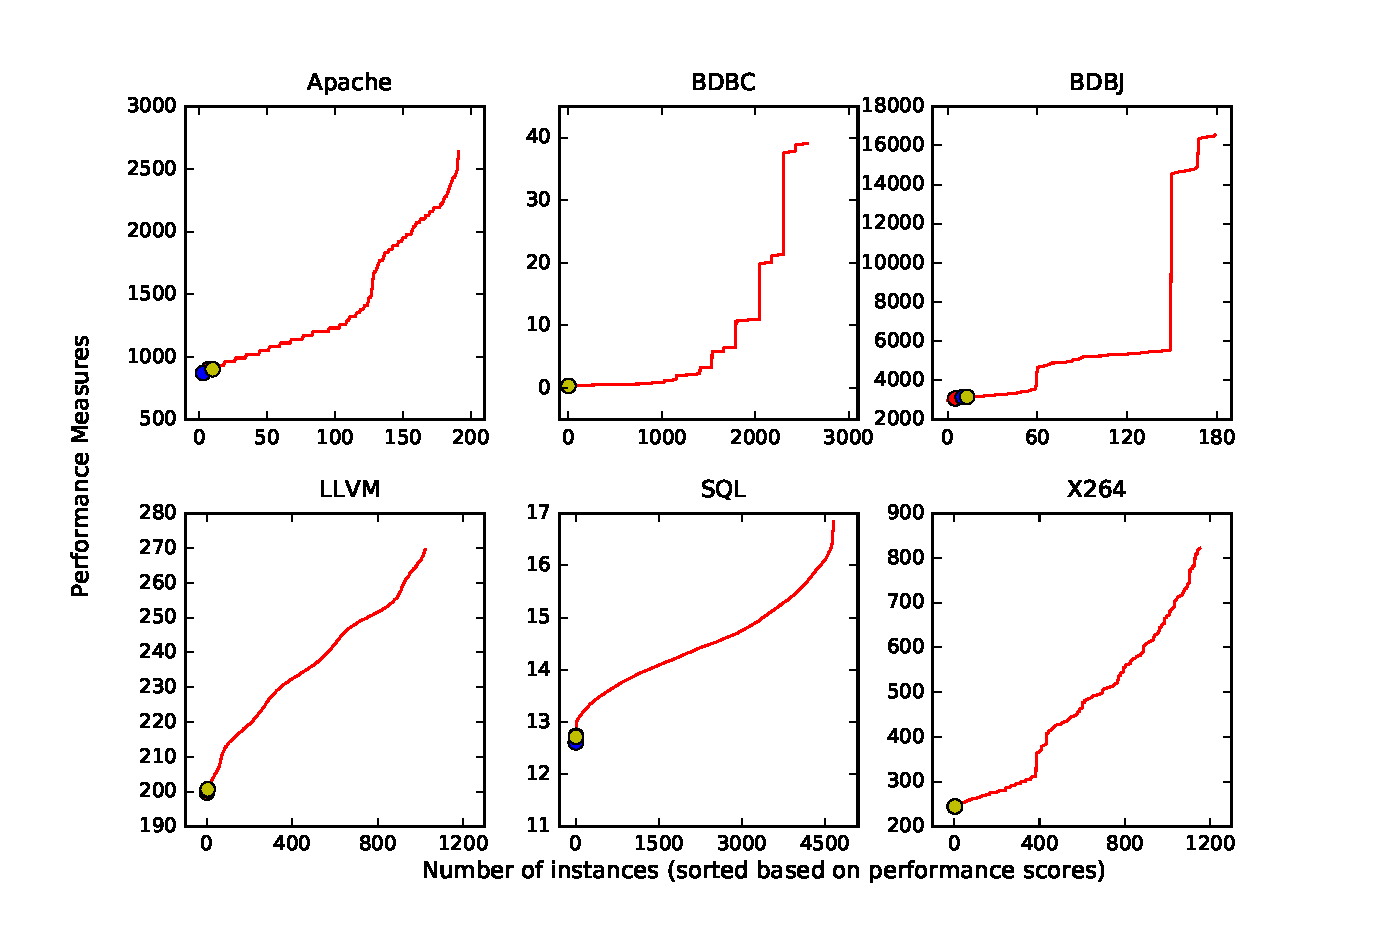
\includegraphics[width=0.9\linewidth]{Figures/optimizer_result.eps}
\caption{Solutions found by GALE}\label{fig:performance_graph}
\end{figure}



We try to answer the following research question in this section\\

\textit{C. Can evolutionary algorithms be used to find the optimal
configurations using the model generated?}
\\
Figure ~\ref{fig:performance_graph} presents the results after running GALE with the performance model. The figure shows the distribution of the performance score (sorted in the ascending order). In the figure we would like to show that GALE has been able to find the configuration/s with minimal performance scores. The green spot on the graphs shows the solution found as the minimum scores. At this point, we would like to point out the GALE doesn't always find the optimal solutions but find solutions close to the optimal. For example, GALE is about to find the third best configuration for SQL lite. We show here that using the software model build using \textit{WHERE east west}, we have been able near optimal solution. We believe that this further validates the usefulness of our approach.  


 
 
\section{Reliability and Validity}\label{sect:construct}


{\em Reliability} refers to the consistency of the results obtained
from the research.  For example,   how well independent researchers
could reproduce the study? To increase external
reliability, this paper has taken care to either  clearly define our
algorithms or use implementations from the public domain
(SciKitLearn). Also, all the data used in this work is available
on-line in the PROMISE code repository and all our algorithms
are on-line at github.com/ai-se/where.


{\em Validity} refers to the extent to which a piece of research actually
investigates what the researcher purports to investigate.
{\em Internal validity} checks if the differences found in
the treatments can be ascribed to the treatments under study. 
One internal validity issue with our experiments is the choice
of {\em training and testing} data sets discussed in 
\tion{design}. Recall that while all our learners used the same
{\em testing} data set, our untuned learners were only given
access to {\em training} while GALE could get feedback from
{\em training} and
{\em tuning}.  

{\em Internal validity}
Regarding SQLite, we cannot measure all possible configurations in reasonable time. Hence, we sampled only 100 configurations to compare prediction and actual performance values. We are aware that this evaluation leaves room for outliers.
Also, we are aware that measurement bias can cause false interpretations [20]. Since we aim at predicting performance for a special workload, we do not have to vary benchmarks.



{\em External validity}  We aimed at increasing the external validity by choosing programs from different domains with different configuration mechanisms and implemented with different programming languages. Furthermore, the programs used are deployed and used in real world. Nevertheless, assuming the evaluations to be automatically transferable  to all configurable programs is not fair. To further strengthen the external validity we run the model(generated by \textit{WHERE east west} against other searchers like NSGAII and differential evolution algorithms\cite{storn1997differential}. This is to validate teh fact that the model doesn't only work for GALE style of perturbation. In Table \ref{external_validity}, we see that the models developed is valid for all searchers, as all searchers are able to find the near optimal solutions.

\begin{table}
\resizebox{3.3 in}{!}{


\begin{tabular}{|l|l|l|l|l|l|l|l|l|l|l|l|l|}
\hline
\multirow{2}{*}{Searcher} & \multicolumn{2}{l|}{Apache} & \multicolumn{2}{l|}{\begin{tabular}[c]{@{}l@{}}Berkeley \\ DB C\end{tabular}} & \multicolumn{2}{l|}{\begin{tabular}[c]{@{}l@{}}Berkeley \\ DB Java\end{tabular}} & \multicolumn{2}{l|}{LLVM} & \multicolumn{2}{l|}{SQL} & \multicolumn{2}{l|}{X264} \\ \cline{2-13} 
                          & Median         & IQR        & Median                                 & IQR                                  & Median                                   & IQR                                   & Median       & IQR        & Median      & IQR        & Median       & IQR        \\ \hline
GALE                      & 870            & 0          & 0.3633                                 & 0.004                                & 3139                                     & 70                                    & 202.23       & 3.98       & 13.1284     & 0.2411     & 247.717      & 3.34       \\ \hline
DE                        & 840            & 0          & 0.3589                                 & 0.002                                & 3139                                     & 70                                    & 199.68       & 0          & 13.079      & 0          & 244.27       & 0.003      \\ \hline
NSGA2                     & 840            & 0          & 0.3536                                 & 0.005                                & 3139                                     & 70                                    & 199.68       & 0          & 13.079      & 0.406      & 244.27       & 0.05       \\ \hline
\end{tabular}}
\caption{The minimum performance scores as found by learners GALE, NSGAII and DE. The scores here show that all the learners are able to find configuration with minimum scores}
\label{external_validity}

\end{table}


{\em Parameter Bias} 
For this study, we did not do extensive parameter tuning:
NSGA-II and DE were run using their default
settings while GALE was run using the settings that
worked well on the first model we studied, which were
then frozen for the rest of this study. As documented
above, those parameters were:
\begin{itemize}
\item $\mu$ = 100: population size;
\item $\omega$ = $\mu$: minimum size leaf clusters;
\item $\lambda$ = 3: premature stopping criteria (sets the maximum
allowed generations without any improvement
on any objective).
\item $\delta$ = 1: the ``accelerator'' that encourages larger
mutations;
\item $\gamma$ = 1.5: the ``brake'' that blocks excessive mutation.
\end{itemize}

If this paper was arguing that these parameters were
somehow optimal, then it would be required to present
experiments defending the above settings. However, our
claim is less than that—we only aim to show that with
these settings, GALE does as well than standard searching
tools. In future work, we will explore other settings.




That said, there exist some class of data mining papers for which
tuning may not be required. Consider  Le Goues et al.'s 2012
ICSE paper that used a evolutionary program to learn
repairs to code~
in that paper was ``can we fix any of the known bugs?''. Note
that this criteria is a ``{\em competency}'' statement, and
not a ``{\em better than}'' statement (the difference being that
one is 
``can do'' and the other is ``can do better''). For such
competency claims, tuning is not necessary. However, as soon
as {\em better than} enters the performance criteria then this
becomes a race between competing methods. In such a race,
it is unfair to hobble one competitor with poor tunings.



\section{Conclusions}

We introduce two new sampling techniques called \textit{WHERE-east-west} and \textit{WHERE exemplar} for performance-prediction of configurable systems. To evaluate and compare the techniques, we used the time saved and prediction accuracy. We conducted empirical studies on six real-world configurable systems to determine an ideal sampling strategy for performance prediction of configurable software system. Our key findings are:
\bi
    \item{Clustering can also be used as a part of the process of sampling and can reduce the number of examples required to train a model}
    \item{Less data does help to build stable models since the variance is always lower than 6\%}
    \item{The model is stable enough so that any optimizer can use the model to find optimal configuration.}
    \item{Using extreme points of the first principle component is a good representative of the entire cluster.}
\ei

Our empirical findings are meant to help the stakeholders in finding optimal configurations to achieve the desired performance scores. In the future...

\section{Future Work}

TO BE FILLED
 
 

\section*{Acknowledgments}
TO BE FILLED
 
\vspace*{0.5mm}
 
 
\bibliographystyle{plain}

\balance
\bibliography{activeconfig}  

   



  


  

\end{document}
 
\subsection{Implications}

time for an end to era of data mining in se? moving on to a new phase of learning-as-optimization

1) learning is actually an optimization tasks (e.g. see fig2 of  learners climbing the roc curve hill in http://goo.gl/x2EaAm)

2) our learners are all contorted to do some tasks X (e.g. minimize expected value of entropy), then we assess them on score Y (recall). which is nuts. maybe we should build the goal predicate into the learner (e.g http://menzies.us/pdf/10which.pdf) 

3) given 1 + 2, maybe the whole paradigm of optimizing param selection is wrong. maybe what we need is a library of bees buzzing around making random choices (e.g. about descritziation) which other bees use, plus their own random choices (e.g. max depth of tree learned from discretized data) which is used by other bees, plus their own random choices (e.g. business users reading the models).  the funky thing here is that it can take some time before some of the bees (the discretizers) get feedback from the community of people using their decision (the tree learners). 




